\documentclass{beamer}

\usefonttheme{professionalfonts} % using non standard fonts for beamer
\usefonttheme{serif} % default family is serif

\usepackage{hyperref}

%\usepackage{minted}

\usepackage{animate}

\usepackage{graphicx}

\def\Put(#1,#2)#3{\leavevmode\makebox(0,0){\put(#1,#2){#3}}}

\usepackage{color}

\usepackage{tikz}

\usepackage{amssymb}

\usepackage{enumerate}


\newcommand\blfootnote[1]{%

  \begingroup

  \renewcommand\thefootnote{}\footnote{#1}%

  \addtocounter{footnote}{-1}%

  \endgroup

}

\makeatletter

%%%%%%%%%%%%%%%%%%%%%%%%%%%%%% Textclass specific LaTeX commands.

 % this default might be overridden by plain title style

 \newcommand\makebeamertitle{\frame{\maketitle}}%

 % (ERT) argument for the TOC

 \AtBeginDocument{%

   \let\origtableofcontents=\tableofcontents

   \def\tableofcontents{\@ifnextchar[{\origtableofcontents}{\gobbletableofcontents}}

   \def\gobbletableofcontents#1{\origtableofcontents}

 }

%%%%%%%%%%%%%%%%%%%%%%%%%%%%%% User specified LaTeX commands.

\usetheme{Malmoe}

% or ...

\useoutertheme{infolines}

\addtobeamertemplate{headline}{}{\vskip2pt}



\setbeamercovered{transparent}

% or whatever (possibly just delete it)

\makeatother

\begin{document}
\title[DCEL report]{RIDIR Report}
\author[AC]{Andres Calderon}
\institute[Fall'19]{University of California, Riverside}
\makebeamertitle
\newif\iflattersubsect

\AtBeginSection[] {
    \begin{frame}<beamer>
    \frametitle{Outline} 
    \tableofcontents[currentsection]  
    \end{frame}
    \lattersubsectfalse
}

\AtBeginSubsection[] {
    \begin{frame}<beamer>
    \frametitle{Outline} 
    \tableofcontents[currentsubsection]  
    \end{frame}
}

\begin{frame}{Working on Edge Partitioner}
{Re-checking DCEL local construction}
    \begin{itemize}
        \item Tunning the prunning of duplicates half edges.
        \item Removing the use of look-up lists.
        \item Worked face assignment base on polygon id.
        \item Dealing with the issue when a cell does not cover any edge.
    \end{itemize}
\end{frame}

\begin{frame}{Working on Edge Partitioner}
{Re-checking DCEL local construction}
    \begin{itemize}
        \item Tunning the prunning of duplicates half edges.
        \item Removing the use of look-up lists.
        \item Improved performance: 
    \end{itemize}
    \centering
    \begin{tabular}{ r r r r }
        \hline
        Dataset & Polygons & Edges & Diff \\ 
        \hline
        CA\_districts\_2000 & 7028 & 999763  & from 5.6s to 2.4s  \\
        CA\_districts\_2010 & 8047 & 2901758 & from 21.5s to 5.4s \\
        \hline
    \end{tabular}    
\end{frame}

\begin{frame}{Working on Edge Partitioner}
{Re-checking DCEL local construction}
    \begin{itemize}
        \item Worked face assignment base on polygon id.
        \begin{itemize}
            \item It does not work because a polygon can have multiples faces in a partition.
            \item Tried to include an additional field or some feature from the polygon to differentiate but there was not gain in performance.
        \end{itemize}
    \end{itemize}
\end{frame}

\begin{frame}{Working on Edge Partitioner}
{Re-checking DCEL local construction}
    \centering 
    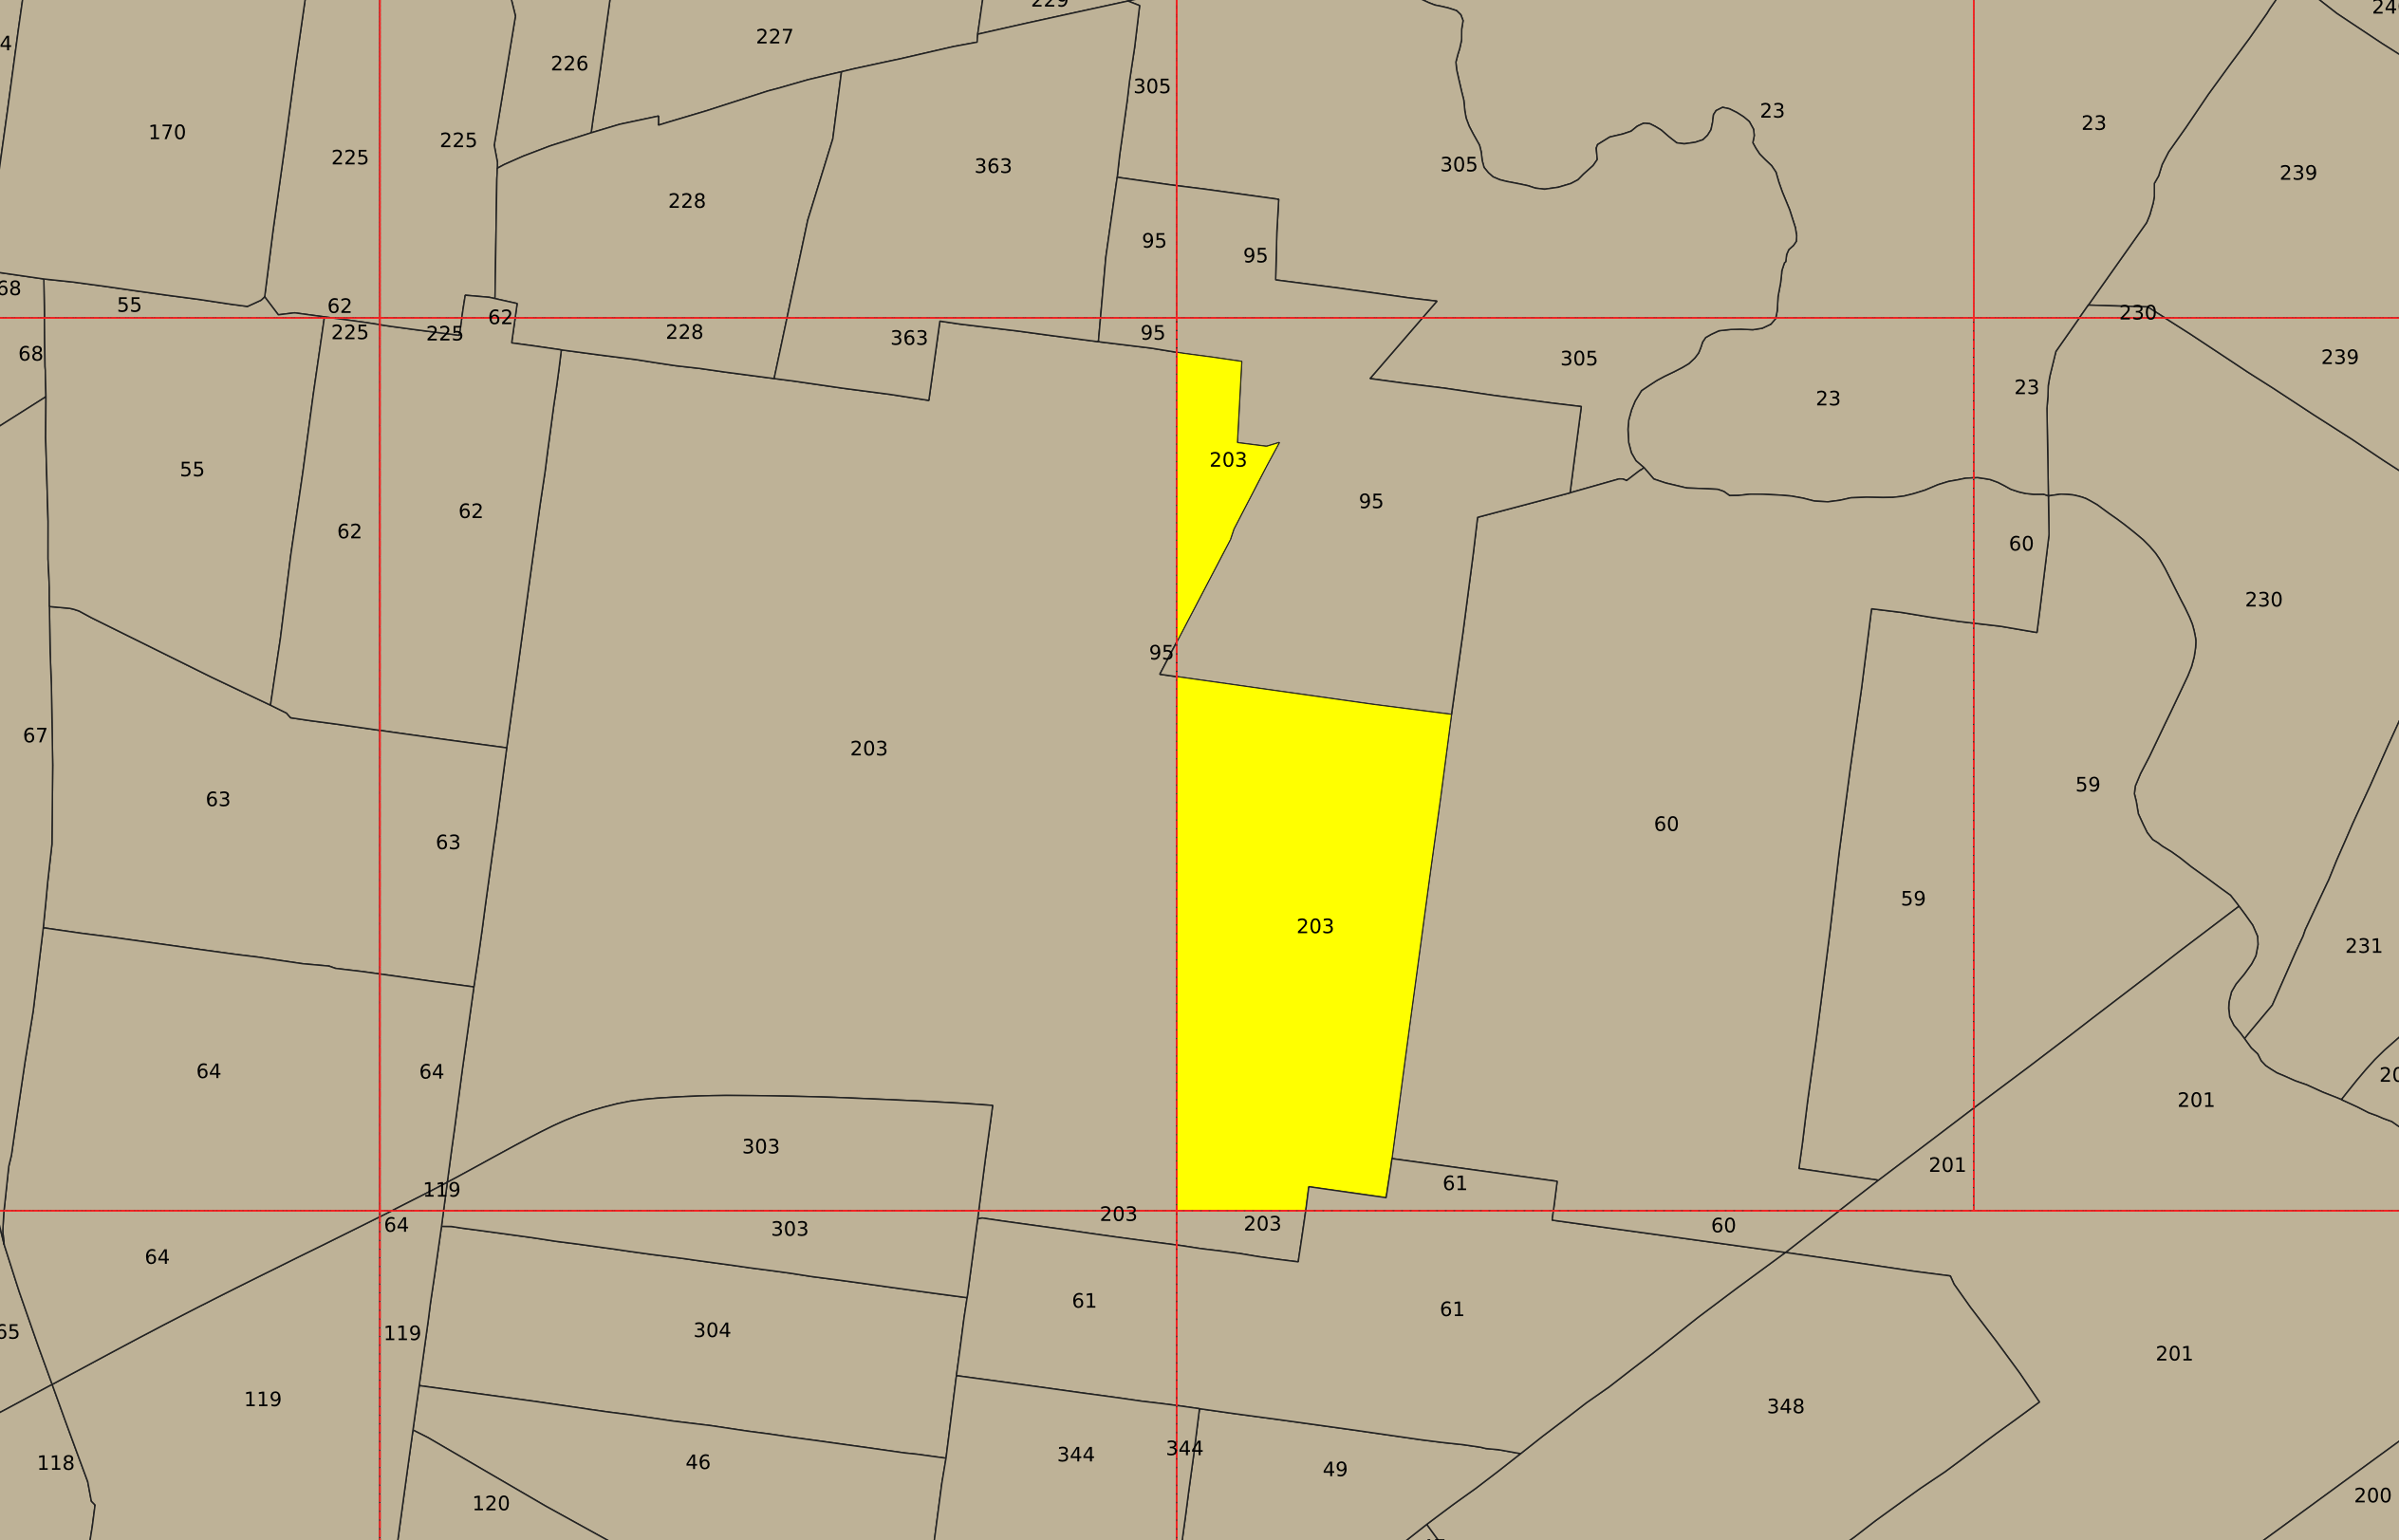
\includegraphics[width=0.8\linewidth]{figures/CA_Faces}     
\end{frame}

\begin{frame}{Working on Edge Partitioner}
{Re-checking DCEL local construction}
    \begin{itemize}
        \item Dealing with the issue when a cell does not cover any edge.
        \item Working on an alternative including the polygon layer to mark those cells which are completely covered by a polygon.
    \end{itemize}
\end{frame}

\begin{frame}{Working on Edge Partitioner}
{Re-checking DCEL local construction}
    \centering 
    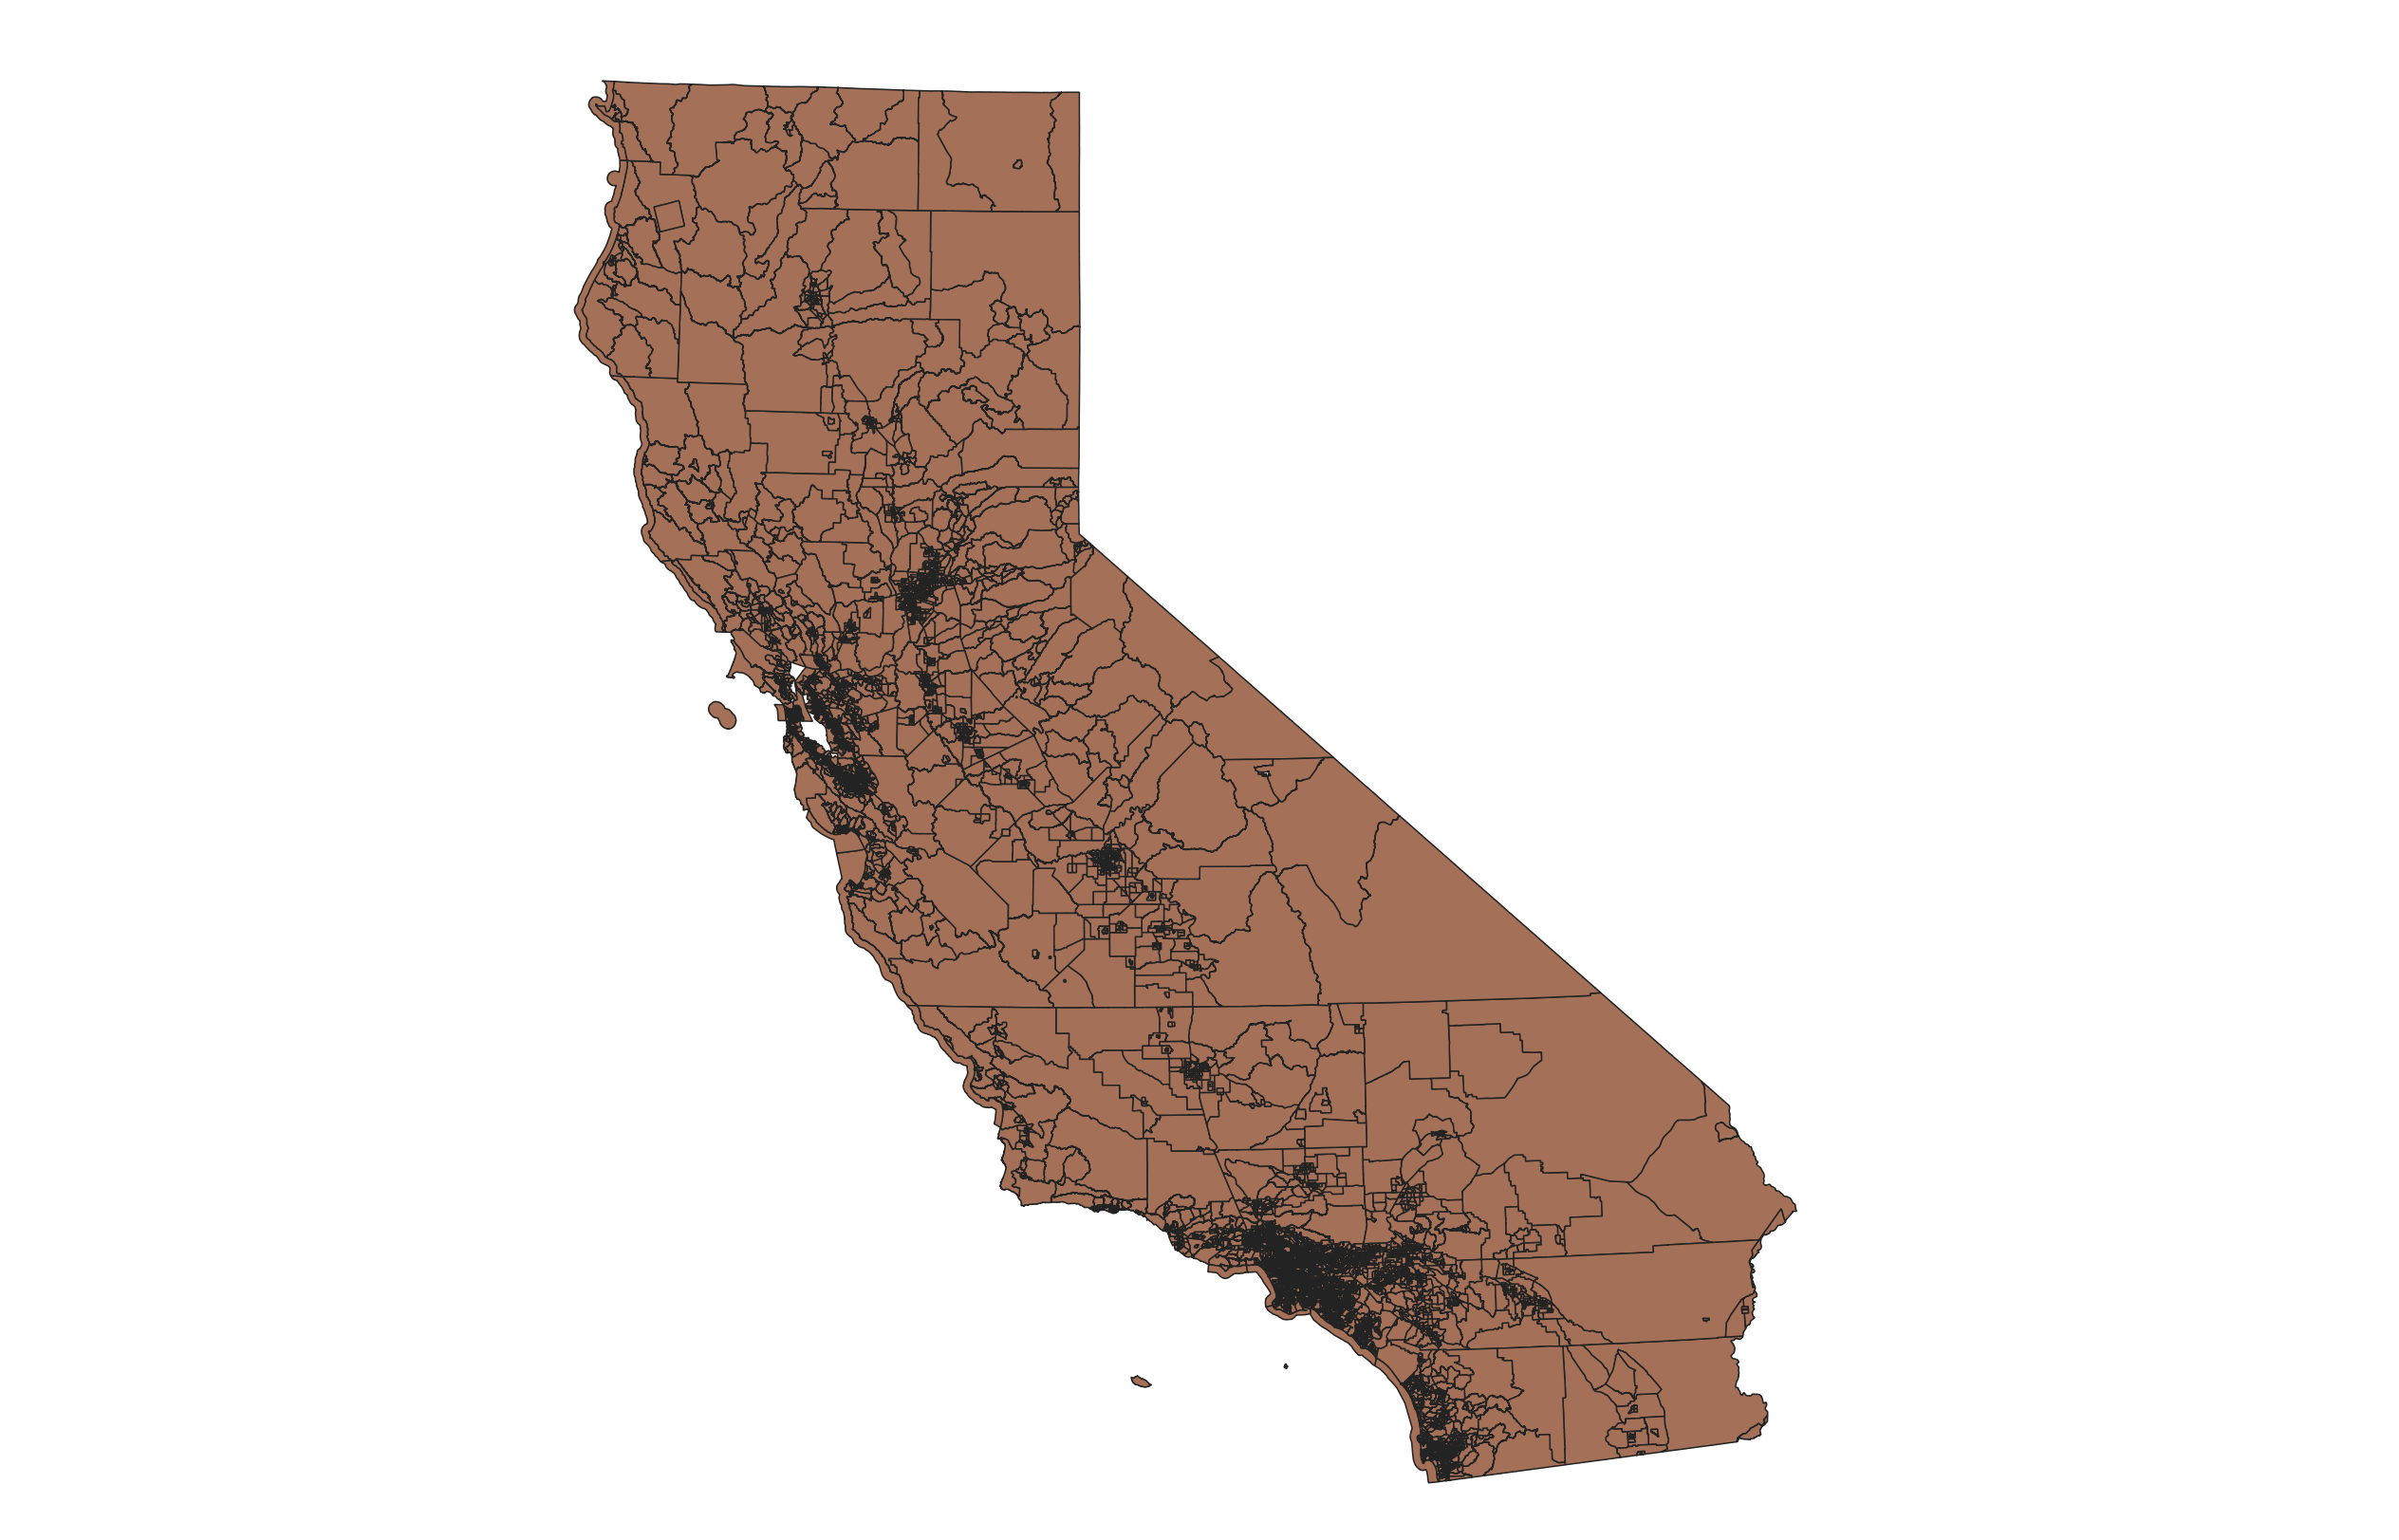
\includegraphics[width=\linewidth]{figures/CA_Cells01}     
\end{frame}

\begin{frame}{Working on Edge Partitioner}
{Re-checking DCEL local construction}
    \centering 
    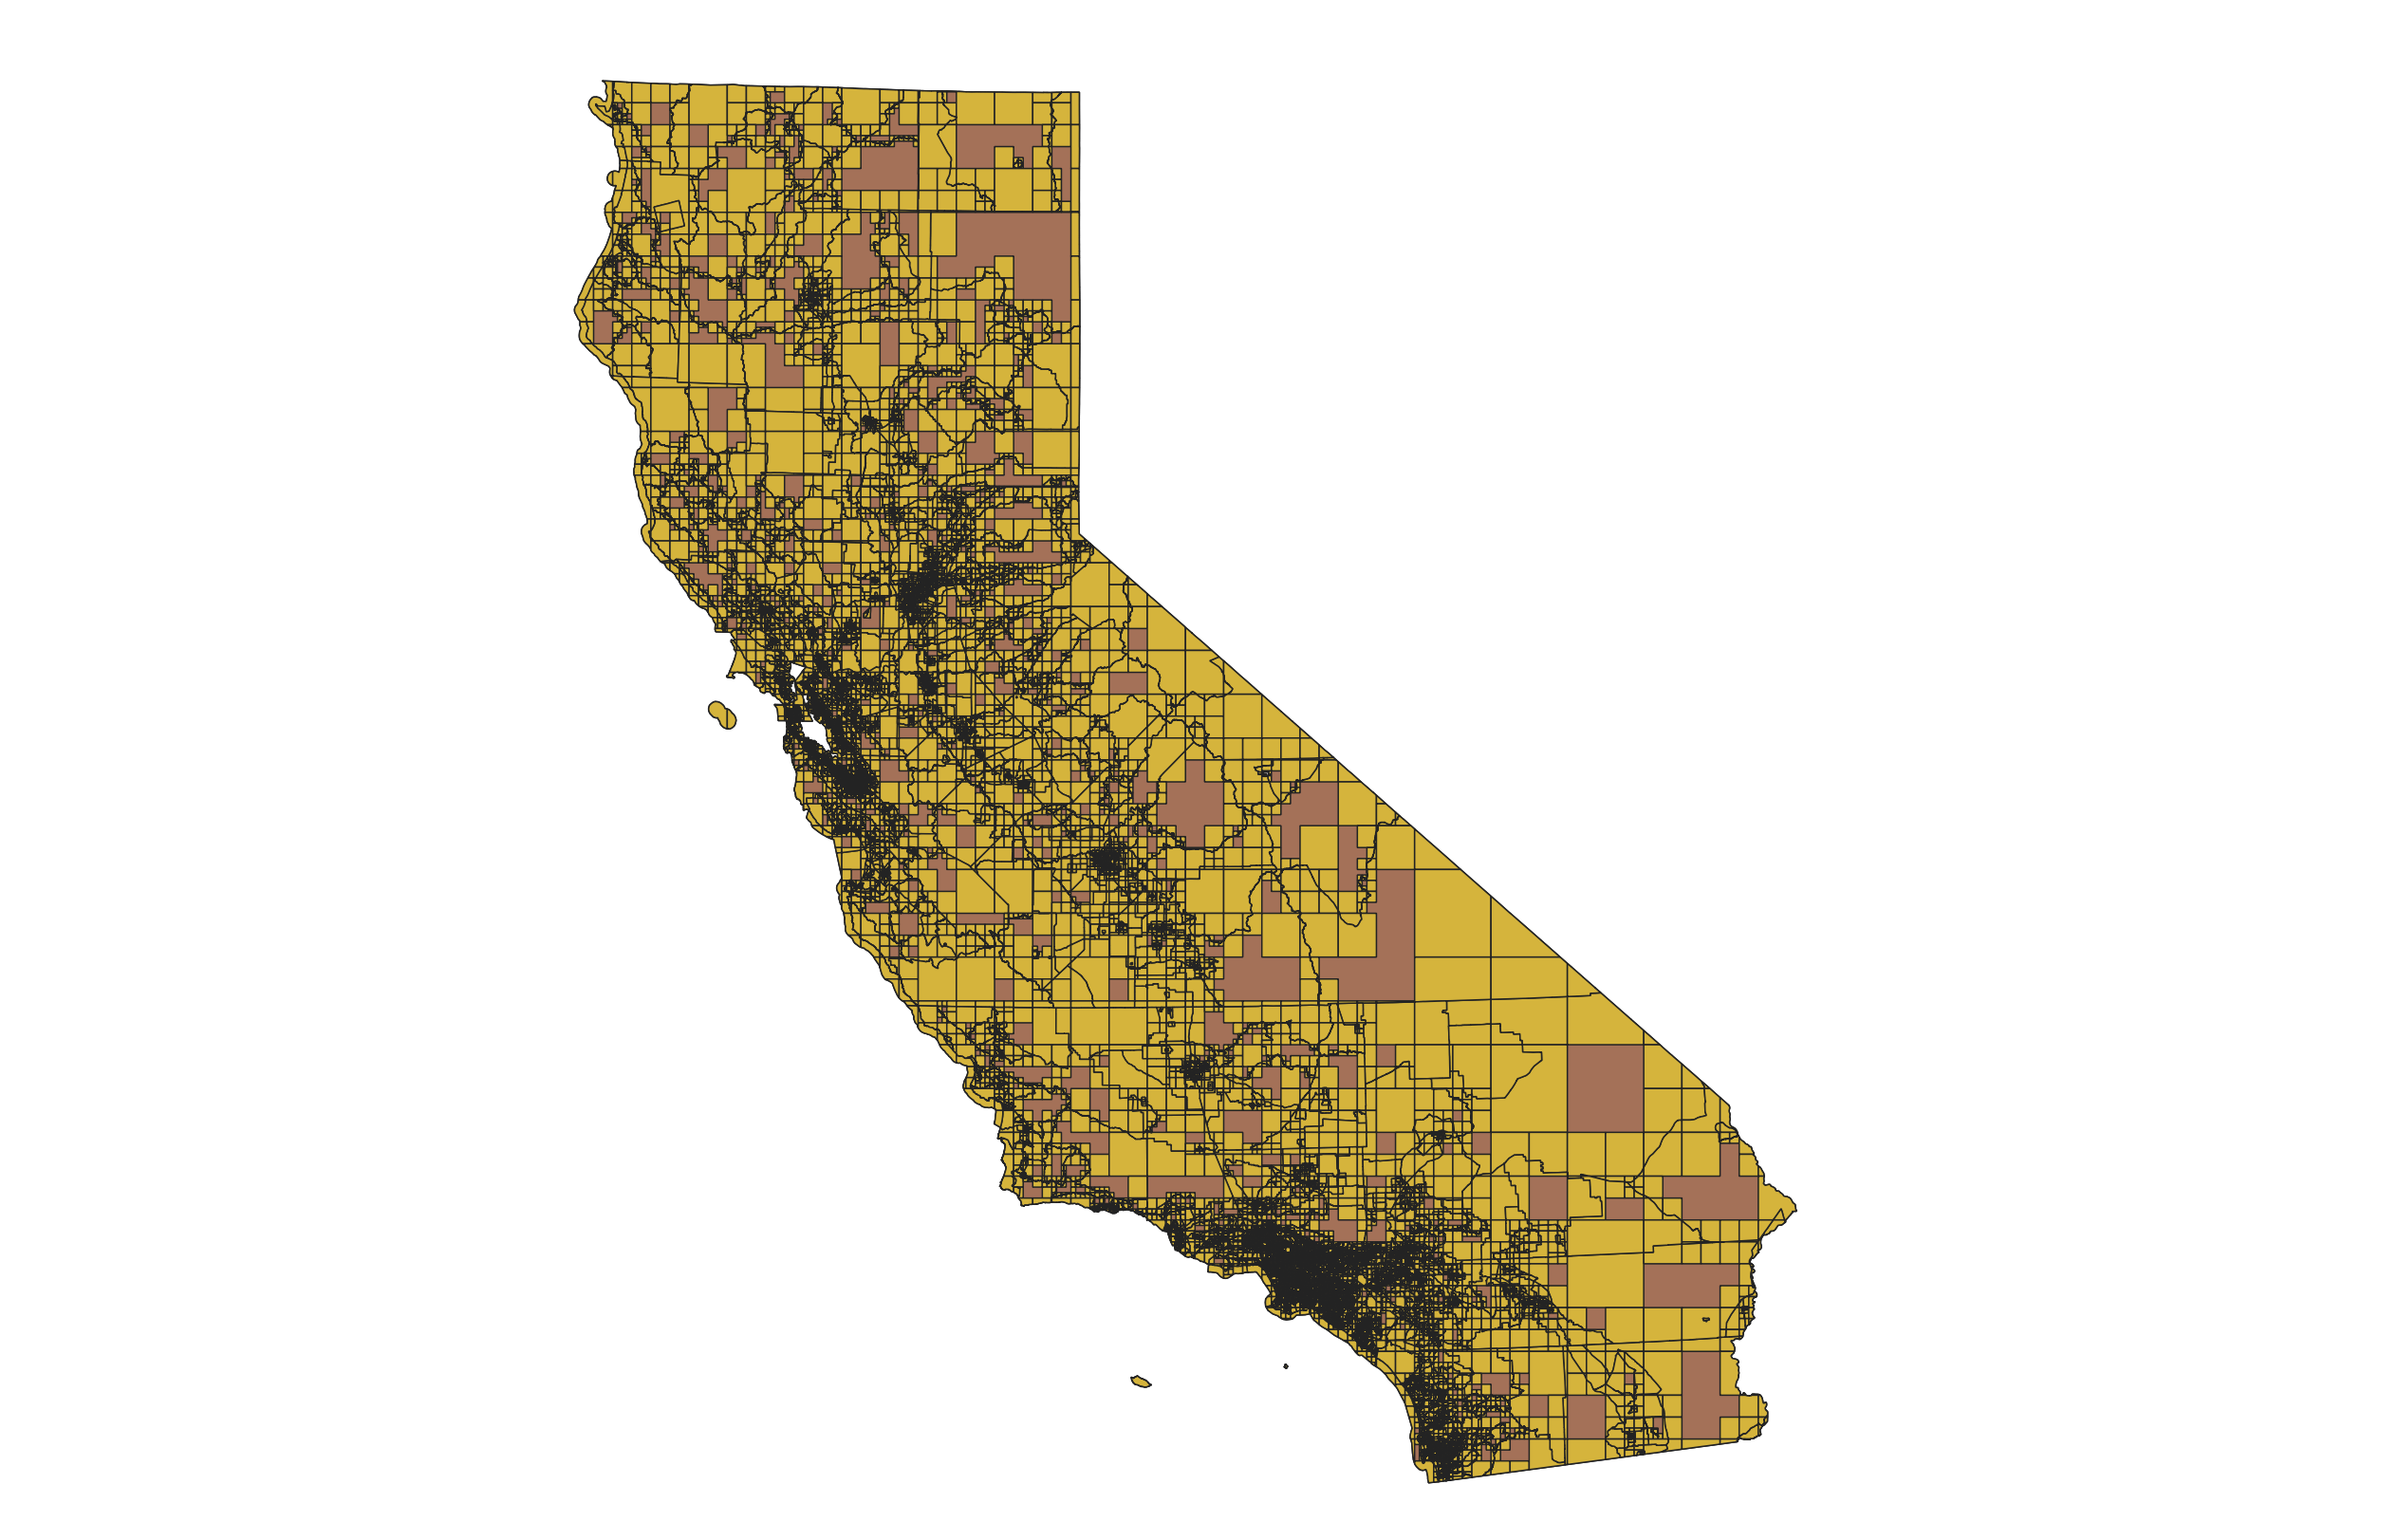
\includegraphics[width=\linewidth]{figures/CA_Cells02}     
\end{frame}

\begin{frame}{What is next?}
    \begin{itemize}
        \item Fix issue with cells and edges.
        \item Re-check improvement versus previous implementation.
        \item Integrate the code.
    \end{itemize}
\end{frame}

\end{document}
